\chapter{Techniques for Adaptive Beamforming}

\indent\indent Here, we discuss three algorithms used for adaptive beamforming. Advantages, disadvantages and a a brief about each algorithm is provided. The final output that is of weight updation is correlated with the beamforming techniques considered. The main considerations include the input signal sample consideration, obtaining minimum variance, minimum Interference to Noise Ratio (INR) (SNR maximisation). Under these conditions, the two main categories considered are the sample by sample based adaptive
techniques and the block adaptive based techniques. Beamformer under these are studied,
implemented and compared under the same signal, noise and interference conditions.

\section{Sample by sample techniques}

The optimal beamformer can be found by techniques that compute the beamforming weights sample by sample and update the weights for each new sample. Over here, least squares problem is solved in a constrained way rather than an unconstrained one which differentiates it from adaptive filters. As a result, we have the steering vector, in contrast to the cross-correlation vector,thus is a priori and is not derived from the data. The main techniques explored under this include least mean square technique and recursive least mean square.

\subsection{Least mean squares}
This type of estimation, minimizes the sum of squares of the estimated error, requires the measurement of both the input signal and the desired response signal. A set of measurements of the desired response y(n) and the input signals xk(n) for k from 1 to M has been taken for n from 0 to N - 1. The task is to estimate the desired response y(n) using the linear combination given as in \ref{eq:1}

\begin{equation} \label{eq:1}
\hat(y)(n) = \sum_{k=1}^{M} c_{k}^{*}x(n) = c^{H}(n)x(n)
\end{equation}

where estimation error is defined as in \ref{eq:2}

\begin{equation} \label{eq:2}
e(n) = y(n) - \hat(y)(n) = y(n) - c^{H}(n)x(n)
\end{equation}

The coefficients of the combiner are hence computed by minimizing the sum of the
squared errors is described as in \ref{eq:3}

\begin{equation} \label{eq:3}
E = \sum_{n=0}^{N-1} |e(n)|^{2}
\end{equation}


\subsection{Recursive least squares}
This technique also revolves about a constrained rather than an unconstrained optimization. Here, y(n) as discussed in the previous section is not the desired response. However, for the adaptive beamformer the steering vector is used, which is deterministic. Algorithms based on RLS methods can be implemented such that the output y(n) is computed directly (direct output extraction) or the adaptive beamformer weights are computed and then applied to determine the output. The RLS methods are based on the update equation of the estimate of the correlation matrix is given as described in \ref{eq:4}

\begin{equation} \label{eq:4}
\hat(R_{x})(n+1) = (\Lambda)_{rls}\hat(R_{x})(n) + x(n+1)x^{H}(n+1)
\end{equation}


where $0 < \lambda_{rls} \le 1$ is a scalar sometimes referred to as the forgetting factor.\vspace{0.75cm}

\section{Block adaptive techniques}
In this techniques, a block of data is used to determine the beamformer weight vectors. The sample matrix inversion fall under this category of technique. The estimates of the statistics used by these methods are based on the data, but they are updated with each block of samples.

\subsection{Sample matrix inversion}
In the real-time context, correlations must be deduced from the incoming data. The ML estimate of the correlation matrix is therefore given by the average of the outer products of the array snapshots: where the indices nk define the K samples of $x_{i} + n(n)$ for 1 n N that make up the training set. The obtained ML estimate of the correlation matrix implies that as K $\rightarrow \infty$, then $R_{i}+n \rightarrow R_{i}+n$. The number K of snapshots utilised to compute the sample correlation matrix is the sample support. The estimate improves with increasing sample size $R_{i+n}$ of the correlation matrix for stationary data. Substituting the sample correlation matrix into the optimum beamformer weight computation as given in \ref{eq:5}

\begin{equation} \label{eq:5}
c_{smi} = \dfrac{\hat(R)_{i+n}^{-1}v(\phi_{S}}{v^{H}(\phi_{s}\hat(R)_{i+n}^{-1}}
\end{equation}


The resulting beampattern obtained from this procedure is defined as the SMI based beamformer.

\section{Choosing adaptive beamforming algortithm}
The electronic scanning unit takes available info (from DOA), feedback from output and generates certain information array factors or weights which adjusts the time delay units and phase shifters to produce desired beam pattern. To compute this weights we require  adaptive beamforming algorithms such as Least mean square(LMS), Recursive Least Square(RLS) or To compute this weights we require  adaptive beamforming algorithms such as Least mean square(LMS), Single Matrix Inversion(SMI) or Recursive Least Square(RLS) as discussed above.

\begin{itemize}
\item LMS is an iterative process which corrects its output by considering the error from previous data but to converge it requires many iterations.
\item SMI  converges faster than LMS as it uses inverse of correlation matrix. But it is computationally complex.
\item RLS encompasses features of both SMI and LMS as it converges faster but has higher margin of error than SMI but lesser than LMS.
\end{itemize}
The targeted hardware that is the FPGA is capable of handling computationally expensive operations and hence, we choose SMI for the implementation of the adaptive beamforming algorithm to get optimal beamformer weights.

\section{MATLAB design for weight calculation}
Regular subarrays are used as antenna elements. Required Frequency, wavelength, spacing between the antenna elements are taken as the design parameters. Signal required to be detected is generated and the jammers as interference signals by using SNR, azimuth angle, elevation angle. Taking the above signals as inputs to the standard SMI Algorithm, optimal beamformer weights are are calculated. It is to be noted that the subarray matrix is using an existing algorithms that leads to a better adaptive beamforming design.

\begin{figure}[H]
\centering
	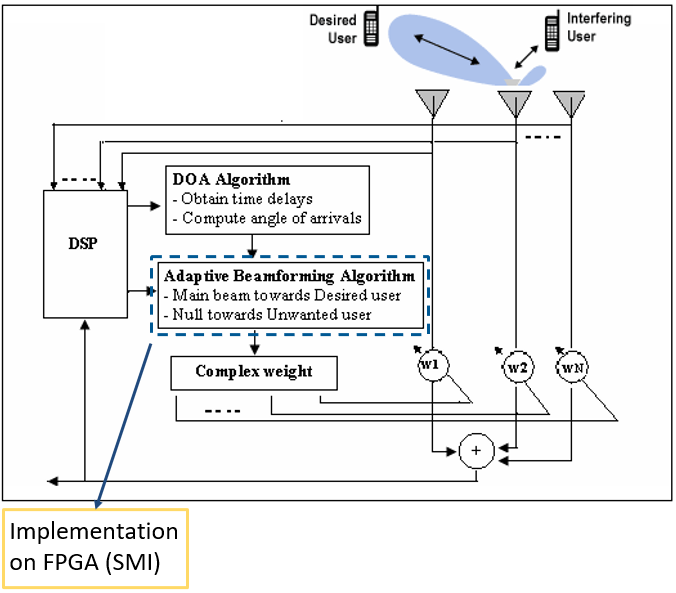
\includegraphics[scale=0.7]{Chapter3/Figures/matlab_algo}	
	\caption{\label{fig:matlab_algo}SMI Algorithm implemented at position shown}
\end{figure}